\documentclass[
11pt, % The default document font size, options: 10pt, 11pt, 12pt
%codirector, % Uncomment to add a codirector to the title page
]{charter} 




% El títulos de la memoria, se usa en la carátula y se puede usar el cualquier lugar del documento con el comando \ttitle
\titulo{Extensión de plataforma de detección RFID Atheling} 

% Nombre del posgrado, se usa en la carátula y se puede usar el cualquier lugar del documento con el comando \degreename
\posgrado{Carrera de Especialización en Sistemas Embebidos} 
%\posgrado{Carrera de Especialización en Internet de las Cosas} 
%\posgrado{Carrera de Especialización en Intelegencia Artificial}
%\posgrado{Maestría en Sistemas Embebidos} 
%\posgrado{Maestría en Internet de las cosas}

% Tu nombre, se puede usar el cualquier lugar del documento con el comando \authorname
\autor{Mag. Ing. Andrade R. Edda G.} 

% El nombre del director y co-director, se puede usar el cualquier lugar del documento con el comando \supname y \cosupname y \pertesupname y \pertecosupname
\director{Esp. Ing. Abbate Santiago}
\pertenenciaDirector{EmTech} 
% FIXME:NO IMPLEMENTADO EL CODIRECTOR ni su pertenencia
\codirector{Falta Definir} % para que aparezca en la portada se debe descomentar la opción codirector en el documentclass
\pertenenciaCoDirector{Falta Definir}

% Nombre del cliente, quien va a aprobar los resultados del proyecto, se puede usar con el comando \clientename y \empclientename
\cliente{Mauro Koenig}
\empresaCliente{EmTech}

% Nombre y pertenencia de los jurados, se pueden usar el cualquier lugar del documento con el comando \jurunoname, \jurdosname y \jurtresname y \perteunoname, \pertedosname y \pertetresname.
\juradoUno{Nombre y Apellido (1)}
\pertenenciaJurUno{pertenencia (1)} 
\juradoDos{Nombre y Apellido (2)}
\pertenenciaJurDos{pertenencia (2)}
\juradoTres{Nombre y Apellido (3)}
\pertenenciaJurTres{pertenencia (3)}
 
\fechaINICIO{22 de agosto de 2023}		%Fecha de inicio de la cursada de GdP \fechaInicioName
\fechaFINALPlan{10 de octubre de 2023} 	%Fecha de final de cursada de GdP
\fechaFINALTrabajo{Julio 2024 (estimada)}	%Fecha de defensa pública del trabajo final


\begin{document}

\maketitle
\thispagestyle{empty}
\pagebreak


\thispagestyle{empty}
{\setlength{\parskip}{0pt}
\tableofcontents{}
}
\pagebreak


\section*{Registros de cambios}
\label{sec:registro}


\begin{table}[ht]
\label{tab:registro}
\centering
\begin{tabularx}{\linewidth}{@{}|c|X|c|@{}}
\hline
\rowcolor[HTML]{C0C0C0} 
Revisión & \multicolumn{1}{c|}{\cellcolor[HTML]{C0C0C0}Detalles de los cambios realizados} & Fecha      \\ \hline
0      & Creación del documento                                 &\fechaInicioName \\ \hline
1      & Se completa hasta el punto 5 inclusive                 & 7 de septiembre de 2023 \\ \hline
2      & Se completa hasta el punto 9 inclusive y se agregan correcciones de la revisión 1  & 14 de septiembre de 2023 \\ \hline
%		  Se puede agregar algo más \newline
%		  En distintas líneas \newline
%		  Así                                                    & dd/mm/aaaa \\ \hline
%3      & Se completa hasta el punto 11 inclusive                & dd/mm/aaaa \\ \hline
%4      & Se completa el plan	                                 & dd/mm/aaaa \\ \hline
\end{tabularx}
\end{table}

\pagebreak



\section*{Acta de constitución del proyecto}
\label{sec:acta}

\begin{flushright}
Buenos Aires, \fechaInicioName
\end{flushright}

\vspace{2cm}

Por medio de la presente se acuerda con la \authorname\hspace{1px} que su Trabajo Final de la \degreename\hspace{1px} se titulará ``\ttitle'', consistirá esencialmente en la implementación de una etapa de autotuning para lograr el uso de la plataforma de detección RFID de Atheling con antenas de distinto alcance, y tendrá un presupuesto preliminar estimado de 825 h de trabajo y \textcolor{red}{\$XXX}, con fecha de inicio \fechaInicioName\hspace{1px} y fecha de presentación pública \fechaFinalName.

Se adjunta a esta acta la planificación inicial.

\vfill

% Esta parte se construye sola con la información que hayan cargado en el preámbulo del documento y no debe modificarla
\begin{table}[ht]
\centering
\begin{tabular}{ccc}
\begin{tabular}[c]{@{}c@{}}Dr. Ing. Ariel Lutenberg \\ Director posgrado FIUBA\end{tabular} & \hspace{2cm} & \begin{tabular}[c]{@{}c@{}}\clientename \\ \empclientename \end{tabular} \vspace{2.5cm} \\ 
\multicolumn{3}{c}{\begin{tabular}[c]{@{}c@{}} \supname \\ Director del Trabajo Final\end{tabular}} \vspace{2.5cm} \\
%\begin{tabular}[c]{@{}c@{}}\jurunoname \\ Jurado del Trabajo Final\end{tabular}     &  & \begin{tabular}[c]{@{}c@{}}\jurdosname\\ Jurado del Trabajo Final\end{tabular}  \vspace{2.5cm}  \\
%\multicolumn{3}{c}{\begin{tabular}[c]{@{}c@{}} \jurtresname\\ Jurado del Trabajo Final\end{tabular}} \vspace{.5cm}                                                                     
\end{tabular}
\end{table}




\section{1. Descripción técnica-conceptual del proyecto a realizar}
\label{sec:descripcion}

Con el crecimiento exponencial de la población mundial, la producción de alimentos cobró una relevancia fundamental en el mundo globalizado y moderno en el que vivimos. Es por ello que la automatización de los procesos productivos resulta de gran interés. 

Abastecer las grandes demandas de la industria cárnica requiere de un exhaustivo trabajo en zonas agrestes de gran extensión. Es por ello que la compañía EmTech desarrolló distintas plataformas marca Atheling, que se encargan de monitorear a los animales de forma automatizada y remota. Los sistemas de Atheling se encuentran instrumentados con múltiples sensores que permiten mantener un registro de los animales. Cada animal es identificado con un único ID (caravana electrónica HDX). Los datos recolectados por las antenas de Atheling se transmiten y procesan de modo tal que el productor tiene todas las variables relevantes disponibles al alcance de dispositivos de uso cotidiano, como un celular. Esto permite la toma de decisiones en tiempo real, fundamentadas en datos concretos, con la finalidad de optimizar la producción.  

En el marco de la aplicación antes mencionada, la compañía EmTech requiere extender la actual plataforma de detección de animales, para lograr obtener una lectura confiable de las caravanas electrónicas portadas por éstos desde distintas antenas y en distintas condiciones ambientales, rediseñándola para incluir un nuevo microprocesador de ultra bajo consumo. El objetivo del proyecto es portar el código al nuevo microprocesador e implementar una etapa de autosintonización que maximice la señal recibida desde las antenas de Atheling de corto y largo alcance. 

El proyecto presentado en este documento es parte del programa de vinculación con empresas y tiene como objetivo implementar la extensión de la plataforma de detección RFID introducida anteriormente, la cual actualmente se encuentra en uso. Para ello es necesario calcular y simular la etapa de autosintonización con ambas antenas (largo y corto alcance), actualizar el diseño del circuito impreso, generar los archivos de fabricación, portar y actualizar el firmware para que el nuevo microprocesador realice la sintonización con ambas antenas. Por último, se requiere realizar pruebas de validación y un informe de sus resultados. El proyecto será llevado a cabo por la autora de este documento en conjunto con colaboradores de la compañía EmTech.

La etapa de autosintonización con las antenas se realiza por medio de un banco de capacitores con llaves, cuya conmutación es comandada por el microcontrolador embebido en la plataforma. Dicho microcontrolador detecta de forma automática la combinación óptima de capacitores para lograr comunicarse con cada antena. En la Figura 1 se muestra un diagrama de bloques de la solución. El color marrón representa la plataforma como es actualmente, mientras que el color azul muestra la propuesta de extensión. En el esquema se proponen cambios en otros módulos de comunicación, cuyo alcance excede al de este trabajo.   





\begin{figure}[htpb]
\centering 
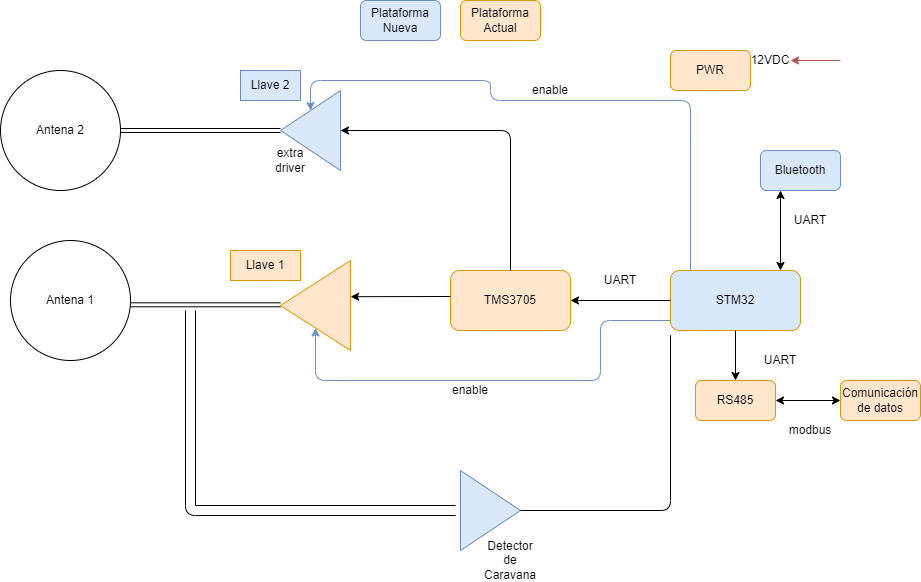
\includegraphics[width=1\textwidth]{./Figuras/Diagrama-de-bloques.png}
\caption{Diagrama en bloques del sistema}
\label{fig:diagBloques}
\end{figure}

\vspace{25px}


\section{2. Identificación y análisis de los interesados}
\label{sec:interesados}



\begin{table}[ht]
%\caption{Identificación de los interesados}
%\label{tab:interesados}
\begin{tabularx}{\linewidth}{@{}|l|X|X|l|@{}}
\hline
\rowcolor[HTML]{C0C0C0} 
Rol           & Apellido y Nombre & Organización 	& Puesto 	\\ \hline
Cliente       & \clientename      &\empclientename	&-       	\\ \hline
Responsable   & \authorname       & FIUBA        	& Alumna 	\\ \hline
Colaboradores & Pedranti Fernando & Atheling      	& Socio    	\\ \hline
Orientador    & \supname	      & \pertesupname 	& Director Trabajo final \\ \hline
%Equipo        & Falta definir
%				          &       -       	& -       	\\ \hline

\end{tabularx}
\end{table}



\section{3. Propósito del proyecto}
\label{sec:proposito}

El propósito de este proyecto es extender el uso de la plataforma de Atheling de detección de animales portadores de caravanas electrónicas para ser utilizada con diferentes antenas, implementado con un microcontrolador de ultra bajo consumo.


\section{4. Alcance del proyecto}
\label{sec:alcance}

El alcance de este proyecto comprende las siguientes actividades:
\begin{itemize}
	\item Simulación y cálculo de la etapa de autosintonización.
	\item Rediseño y fabricación de un prototipo.
	\item Adaptación del firmware al nuevo microcontrolador de ultra bajo consumo.
	\item Actualización del firmware para que el microcontrolador realice de forma automática la sintonización con cada antena.
	\item Planificar y realizar las pruebas de validación del prototipo.
	\item Elaborar un informe de validación del circuito actualizado.
\end{itemize}
Como se especifica en la lista anterior, este proyecto no pretende entregar un equipo integrado en funcionamiento listo para su comercialización sino un prototipo. Cabe mencionar que todas las actividades enlistadas no son responsabilidad exclusiva de la autora de este documento, sino que serán realizadas en conjunto con colaboradores y miembros del equipo de la compañía EmTech-Atheling. 

\section{5. Supuestos del proyecto}
\label{sec:supuestos}

Para lograr el éxito de este proyecto se realizan las siguientes suposiciones:

\begin{itemize}
	\item EmTech realizó una primera aproximación de cálculo para corroborar que el hardware actual sea compatible con la aplicación requerida.
	\item EmTech define los requerimientos detallados y el criterio de aceptabilidad de los entregables.
	\item EmTech pone a disposición toda la información necesaria, con el nivel de detalle adecuado.
	\item La alumna y todos las personas involucradas acuerdan la dinámica laboral, realizando un desgloce de tareas, asignándolas a quien corresponda. 
	\item EmTech asigna los recursos humanos competentes para llevar a cabo el re-diseño y fabricación del prototipo en un plazo de tiempo acotado (falta acordar dicho plazo con la compañía).
	\item EmTech financia la fabricación del prototipo.
	\item EmTech pone a disposición el Hardware necesario para realizar las pruebas de validación del prototipo.
	\item El Director de Proyecto asignado tiene las competencias y la disponibilidad de tiempo necesarios para guiar a la alumna en las tareas específicas de este proyecto. 
	\item La alumna dispone de tiempo para dedicar al proyecto de no menos de 10hs semanales hasta su culminación.
	
\end{itemize}


\section{6. Requerimientos}
\label{sec:requerimientos}


\begin{enumerate}
	\item Requerimientos generales de funcionalidad
	El sistema debe:
		\begin{enumerate}
			\item  Leer etiquetas RFID HDX bajo el estándar ISO 11785.
			\item  Sintonizar automáticamente de la etapa de radiofrecuencia para lectura de las etiquetas.
			\item  Leer las etiquetas hasta una distancia máxima de 60 cm.
			\item  Indicar mediante un estímulo sonoro la correcta lectura de una etiqueta.
			\item  Implementar una comunicación MODBUS vía RS485 para la recepción de comandos de control y lectura de datos.
			\item  Comandar una salida a relé normal abierta, vía la recepción de un comando a través de la interfaz MODBUS.
			\item  Contar con la posibilidad de utilizar una o dos antenas, configurable vía selectores en el PCB.

		\end{enumerate}
	\item Requerimientos de desarrollo del prototipo 
		\begin{enumerate}
			\item El desarrollo del prototipo se basará en la plataforma de lectura Atheling RFID V1.
			\item La decodificación de las etiquetas deberá implementarse con base en el circuito integrado TMS3705.
			\item El control y procesamiento de datos del sistema debe basarse en un microcontrolador STM32L152CBT6.
			\item La plataforma debe contar con una interfaz para su programación mediante un programador externo, sugerencia no estricta: USB ST-Link.
			\item Se deben mantener las dimensiones 2D y fijaciones de la plataforma Atheling RFID V1.
			\item Se deben implementar cambios en el circuito de potencia y en el tamaño de los agujeros
			
		\end{enumerate}
	\item Requerimientos de firmware
	\begin{enumerate}
			\item Portar y/o rehacer el firmware actual para que funcione en el nuevo microcontrolador. 
			\item Desarrollar el código para autosintonización.
			\item Desarrollar drivers para las interfaces de programación, Módulo BLE, RS485, otros periféricos como alarmas sonoras, llaves, etc.
			\end{enumerate}
	\item Requerimientos de control de cambios
	\begin{enumerate}
			\item Se debe mantener actualizadas las versiones de código mediante el uso del repositorio de EmTech.
			\end{enumerate}
	
	\item Requerimientos documentales
	\begin{enumerate}
			\item Se deberá realizar la documentación de desarrollo del código de acuerdo a los lineamientos de documentación de EmTech. 
			\end{enumerate}
			\item Requerimientos de validación y pruebas
	\begin{enumerate}
			\item Se deberá validar el funcionamiento del prototipo mediante pruebas de laboratorio que simulen escenarios de uso la plataforma.
			\end{enumerate}
\end{enumerate}



\section{7. Historias de usuarios (\textit{Product backlog})}
\label{sec:backlog}

En el siguiente párrafo se describe lo expresado por Mauro Koeing, impulsor del proyecto: "Como impulsor del proyecto quiero contar con una etapa automática de sintonización del lector con las antenas para poder utilizar la plataforma en ambientes con diversas condiciones de ruido electromagnético. También quiero mejorar la conectividad de la actual versión y agregar la opción para la utilización de más de una antena."


\section{8. Entregables principales del proyecto}
\label{sec:entregables}

Los entregables del proyecto son:

\begin{itemize}
	\item Documento de ingeniería de la aplicación del circuito, análisis de lo que se agrega, fundamentos y líneas para hacer el esquemático + PCB.
    \item Documentos de fabricación del PCB (Gerbers + archivo de fabricación + P and P).
    \item Esquemáticos del PCB + BOM.
	\item Código fuente del firmware.
	\item Documentación del código.
	\item Informe de cierre del proyecto.

\end{itemize}


\section{9. Desglose del trabajo en tareas}
\label{sec:wbs}

\begin{enumerate}
\item Planificación del proyecto: 78 h
	\begin{enumerate}
	\item Definir el alcance del proyecto: 10 h
	\item Acordar metodologías de trabajo, gestión de la información, medios de comunicación: 20 h
	\item Gestionar los recursos para asegurar la disponibilidad en el momento de realización de las pruebas: 40 h
	\item Confeccionar el Plan de Trabajo: 48 h
	\end{enumerate}

\item Simulación y cálculo de la etapa de autosintonización: 45 h
	\begin{enumerate}
	\item Investigar el estado del arte: 40 h
	\item Calcular el circuito: 20 h
	\item Simular el comportamiento del circuito: 20 h 
	\end{enumerate}
	
\item Diseño del prototipo: 141 h
	\begin{enumerate}
	\item Selecionar los componentes: 20 h
	\item Calcular los circuitos: 10 h
	\item Diseñar los circuitos esquemáticos: 20 h
	\item Confeccionar memorias de cálculo: 10 h
	\item Confeccionar Bill Of Materials (BOM): 5 h
	\item Confeccionar esquemáticos entregables: 20 h
	\item Diseñar el PCB: 40 h
	\item Confeccionar documentos de fabricación (gerbers, Pick and Place, etc.): 10 h
	\item Modelar CAD 3D del PCB: 5 h
	\item Verificar la compatibilidad mecánica/espacial del PCB dentro del gabinete: 1 h
	\end{enumerate}
	
\item Fabricación del prototipo: 120 h
	\begin{enumerate}
	\item Buscar proveedores y solicitar cotizaciones: 20 h
	\item Rediseñar el PCB en función de la retroalimentación con el/los fabricantes: 10 h
	\item Dar seguimiento a la fabricación: 10 h
	\item Fabricar el PCB y montar componentes: 40 h
	\item Integrar el sistema embebido al gabinete, con sus fijaciones, fuente de alimentación, etc.: 40 h
    \end{enumerate}
    
\item Desarrollo de Firmware: 172 h
	\begin{enumerate}
	\item Estudiar el código actual: 10 h
	\item Evaluar si recodificar completamente el código o portar: 2 h
	\item Portar/recodificar las funcionalidades actuales para que funcionen en el nuevo microcontrolador: 40 h
	\item Desarrollar drivers para las interfaces de comunicación, programación y periféricos como alarma sonora: 80 h
	\item Desarrollar el código de autosintonización: 40 h
	\end{enumerate}

\item Prueba del firmware: 45 h
    \begin{enumerate}
    \item Montar periféricos de prueba para verificación de funcionamiento del firmware: 5 h
    \item Analizar y depurar el código: 40 h
    \end{enumerate}

\item Diseño de pruebas de validación: 19 h
    \begin{enumerate}
    \item Definir criterios de aceptación del comportamiento de la plataforma: 20 h
    \item Definir el alcance de las pruebas a realizarse: 2 h
    \item Definir los recursos necesarios (espacio, instrumentación, personal, etc): 5 h
    
    \end{enumerate}
    
\item Pruebas de validación: 70 h
    \begin{enumerate}
    \item Realizar pruebas de validación: 60 h
    \item Documentar pruebas de validación: 10 h
    \end{enumerate}
    
\item Presentación final del proyecto: 89 h
    \begin{enumerate}
    \item Confeccionar el informe de avance: 30 h
    \item Confeccionar las memorias del proyecto: 30 h
    \item Confeccionar la presentación pública: 20 h
    \item Practicar la presentación en conjunto con el director: 5 h
    \end{enumerate}

  
\end{enumerate}


\section{10. Diagrama de Activity On Node}
\label{sec:AoN}

\begin{consigna}{red}
Armar el AoN a partir del WBS definido en la etapa anterior. 

%La figura \ref{fig:AoN} fue elaborada con el paquete latex tikz y pueden consultar la siguiente referencia \textit{online}:

%\url{https://www.overleaf.com/learn/latex/LaTeX_Graphics_using_TikZ:_A_Tutorial_for_Beginners_(Part_3)\%E2\%80\%94Creating_Flowcharts}

\end{consigna}

\begin{figure}[htpb]
\centering 
\includegraphics[width=.8\textwidth]{./Figuras/AoN.png}
\caption{Diagrama de \textit{Activity on Node}.}
\label{fig:AoN}
\end{figure}

Indicar claramente en qué unidades están expresados los tiempos.
De ser necesario indicar los caminos semicríticos y analizar sus tiempos mediante un cuadro.
Es recomendable usar colores y un cuadro indicativo describiendo qué representa cada color, como se muestra en el siguiente ejemplo:



\section{11. Diagrama de Gantt}
\label{sec:gantt}

\begin{landscape}
%\rotatebox{90}{%
\begin{ganttchart}[
	hgrid,
vgrid,
	x unit=0.15cm,
	y unit chart=0.85cm,
time slot format=isodate,
time slot unit=day,
bar/.append style={fill=cyan!30},
group/.append style={fill=magenta!50},
bar/.append style={fill=cyan!30, bar label node/.append style={above=3pt}},
%include title in canvas=false,
%inline,
milestone inline label node/.append style={left=5mm}
%link/.style={->, thick}
%link label font=\small\bfseries\color{purple}
link/.style={|-to, line width=0.5pt, magenta},
    bar inline label node/.style={
	anchor=east,
	xshift=+4.5cm,
	yshift=0.4cm,
}]{2023-08-22}{2023-12-16}
	
%{\small
	\gantttitlecalendar{year, month} \\
	
	\ganttgroup{1 Planificación del Proyecto}{2023-08-22}{2023-10-10} \\
	\ganttbar[name=11]{1.1 Definir el alcance del proyecto}{2023-08-22}{2023-08-30} \\
	\ganttbar[name=12]{1.2 Acordar metodologías de trabajo}{2023-09-01}{2023-09-10} \\
	\ganttbar[name=13]{1.3 Gestionar los recursos}{2023-08-22}{2023-10-10} \\
	\ganttbar[name=14]{1.4 Confeccionar el Plan de Trabajo}{2023-08-22}{2023-10-10} \\
	
	\ganttmilestone{Presentación del Plan de Trabajo}{2023-10-10}\\ 	
	
	\ganttgroup{2 Simulación y cálculo}{2023-10-16}{2023-12-16} \\
	\ganttbar[name=21]{2.1 Investigar el estado del arte}{2023-10-16}{2023-11-15} \\
	\ganttbar[name=22]{2.2 Calcular el circuito}{2023-11-18}{2023-12-02} \\
	\ganttbar[name=23]{2.3 Simular el comportamiento del circuito}{2023-12-02}{2023-12-16} \\
	
	\ganttlink[]{21}{22}
	\ganttlink[]{22}{23}

\end{ganttchart}
%}
%\end{landscape}


%\begin{landscape}
%\rotatebox{90}{%
\newpage
\begin{ganttchart}[
	hgrid,
vgrid,
	x unit=0.15cm,
	y unit chart=0.85cm,
time slot format=isodate,
time slot unit=day,
bar/.append style={fill=cyan!30},
group/.append style={fill=magenta!50},
bar/.append style={fill=cyan!30, bar label node/.append style={above=3pt}},
%include title in canvas=false,
%inline,
milestone inline label node/.append style={left=5mm}
%link/.style={->, thick}
%link label font=\small\bfseries\color{purple}
link/.style={|-to, line width=0.5pt, magenta},
    bar inline label node/.style={
	anchor=east,
	xshift=+4.5cm,
	yshift=0.4cm,
}]
{2023-12-16}{2024-04-10}
	
	\gantttitlecalendar{year, month} \\
	
	\ganttgroup{3 Diseño del prototipo}{2023-12-18}{2024-02-09}\\
	\ganttbar[name=31]{3.1 Seleccionar los componentes}{2023-12-18}{2023-12-20} \\
	\ganttbar[name=32]{3.2 Calcular circuitos}{2023-12-20}{2023-12-21} \\
	\ganttbar[name=33]{3.3 Diseñar esquemáticos}{2024-01-02}{2024-01-04} \\
	\ganttbar[name=34]{3.4 Confeccionar memorias}{2024-01-04}{2024-01-05} \\
	\ganttbar[name=35]{3.5 Confeccionar BOM}{2024-01-05}{2024-01-06} \\
	\ganttbar[name=36]{3.6 Confeccionar de esquemáticos entregables}{2024-01-08}{2024-01-10} \\
	\ganttbar[name=37]{3.7 Diseñar el PCBs}{2024-01-10}{2024-02-07} \\
	\ganttbar[name=38]{3.8 Confeccionar documentos de fabricación}{2024-02-07}{2024-02-08}\\
	\ganttbar[name=39]{3.9 Modelar 3D del PCB}{2024-02-08}{2024-02-09} \\
	\ganttbar[name=310]{3.10 Verificar la compatibilidad mecánica}{2024-02-09}{2024-02-09} \\
	
	
	\ganttgroup{4 Fabricación del prototipo}{2024-02-09}{2024-04-07} \\
	\ganttbar[name=31]{4.1 Gestión de compras}{2024-02-09}{2024-02-15} \\
	\ganttbar[name=42]{4.2 Rediseñar el PCB}{2024-02-09}{2024-02-15} \\
	\ganttbar[name=43]{4.3 Dar seguimiento a la fabricación}{2024-02-15}{2024-03-07} \\
    \ganttbar[name=44]{4.4 Montaje y puesta en marcha inicial}{2024-03-07}{2024-04-07} \\
	\ganttbar[name=45]{4.5 integrar el sistema embebido}{2024-03-07}{2024-04-07} \\
	\ganttmilestone{Prototipo Integrado con HW funcionando}{2024-04-07}\\

\ganttlink[]{31}{32}
\ganttlink[]{32}{33}
\ganttlink[]{32}{34}
\ganttlink[]{35}{37}	
\ganttlink[]{37}{38}
\ganttlink[]{39}{310}
\end{ganttchart}
%}
%\end{landscape}


%\begin{landscape}
%\rotatebox{90}{%
\newpage
\begin{ganttchart}[
	hgrid,
vgrid,
	x unit=0.15cm,
	y unit chart=0.85cm,
time slot format=isodate,
time slot unit=day,
bar/.append style={fill=cyan!30},
group/.append style={fill=magenta!50},
bar/.append style={fill=cyan!30, bar label node/.append style={above=3pt}},
%include title in canvas=false,
%inline,
milestone inline label node/.append style={left=5mm}
%link/.style={->, thick}
%link label font=\small\bfseries\color{purple}
link/.style={|-to, line width=0.5pt, magenta},
    bar inline label node/.style={
	anchor=east,
	xshift=+4.5cm,
	yshift=0.4cm,
}
]{2024-04-07}{2024-06-28}

	
	\gantttitlecalendar{year, month} \\
	
	\ganttgroup{5 Desarrollo de Firmware}{2024-04-07}{2024-05-28} \\
	\ganttbar[name=51]{5.1 Estudiar el código actual}{2024-04-07}{2024-04-08} \\
	\ganttbar[name=52]{5.2 Evaluar si recodificar o portar}{2024-04-08}{2024-04-11} \\
	\ganttbar[name=53]{5.3 Portar/recodificar las funcionalidades actuales}{2024-04-08}{2024-04-30} \\
	\ganttbar[name=54]{5.4 Desarrollar drivers}{2024-04-30}{2024-5-10}\\
	\ganttbar[name=55]{5.5 Desarrollar código de autosintonización}{2024-05-10}{2024-05-27} \\
	\ganttmilestone[name=56]{Presentación al cliente del Código}{2024-05-28} \\
	
	\ganttgroup{6 Prueba del firmware}{2024-04-07}{2024-06-07}\\
	\ganttbar[name=61]{6.1 Montar periféricos de prueba 
}{2024-04-07}{2024-04-30} \\
	\ganttbar[name=62]{6.2 Prueba de FW y corrección de bugs}{2024-05-28}{2024-06-07} \\

	\ganttlink[]{51}{52}
	\ganttlink[]{52}{53}
	\ganttlink[]{52}{54}
	\ganttlink[]{53}{55}
	\ganttlink[]{56}{61}
	\ganttlink[]{61}{62}

	


\end{ganttchart}
%\end{landscape}
%}


%\rotatebox{90}{%
\newpage
%\begin{landscape}
\begin{ganttchart}[
	hgrid,
	vgrid,
	x unit=0.25cm,
	y unit chart=1cm,
	time slot format=isodate,
	time slot unit=day,
	bar/.append style={fill=cyan!30},
	group/.append style={fill=magenta!50},
	link/.style={->, thick}
	]{2024-05-28} {2024-08-03}
	
	\gantttitlecalendar{year, month} \\

\ganttgroup{7 Diseño de pruebas de validación}{2024-05-28}{2024-06-07} \\
	\ganttbar[name=71]{7.1 Definir criterios de aceptación}{2024-05-28}{2024-06-02} \\
	\ganttbar[name=72]{7.2 Definir el alcance de las pruebas}{2024-06-02}{2024-06-03} \\
	\ganttbar[name=73]{7.3 Definir los recursos necesarios}{2024-06-03}{2024-06-03}  \\

	
	\ganttgroup{8 Pruebas de validación}{2024-06-08}{2024-07-08} \\
	\ganttbar[name=81]{8.1 Realizar pruebas de validación}{2024-06-08}{2024-07-07} \\
	\ganttmilestone{Culminación de las pruebas de validación}{2024-07-07} \\
	\ganttbar[name=82]{8.2 Documentar pruebas de validación}{2024-07-07}{2024-07-08}\\
	
	
	
	
	\ganttgroup{9 Presentación final del proyecto}{2024-07-07}{2024-08-01} \\
	\ganttbar[name=91]{9.1 Confeccionar el informe de avance}{2024-07-07}{2024-07-15} \\
	\ganttmilestone{Presentación del Avance del Proyecto}{2024-07-20} \\
	\ganttbar[name=92]{9.2 Confeccionar las memorias del proyecto}{2024-07-07}{2024-07-21} \\
	\ganttbar[name=93]{9.3 Confeccionar la presentación pública}{2024-07-21}{2024-07-28} \\
	\ganttbar[name=94]{9.4 Practicar presentación}{2024-07-28}{2024-07-29} \\
	\ganttmilestone{Defensa Pública del Proyecto}{2024-08-01}
\end{ganttchart}
\end{landscape}
%}
	

\section{12. Presupuesto detallado del proyecto}
\label{sec:presupuesto}
\begin{table}[htpb]
\centering
\begin{tabularx}{\linewidth}{@{}|X|c|r|r|@{}}
\hline
\rowcolor[HTML]{C0C0C0} 
\multicolumn{4}{|c|}{\cellcolor[HTML]{C0C0C0}COSTOS DIRECTOS} \\ \hline
\rowcolor[HTML]{C0C0C0} 
Descripción &
  \multicolumn{1}{c|}{\cellcolor[HTML]{C0C0C0}Cantidad} &
  \multicolumn{1}{c|}{\cellcolor[HTML]{C0C0C0}Valor unitario} &
  \multicolumn{1}{c|}{\cellcolor[HTML]{C0C0C0}Valor total} \\ \hline
 & 
  \multicolumn{1}{c|}{837} &
  \multicolumn{1}{c|}{20} &
  \multicolumn{1}{c|}{16740} \\ \hline
  \multicolumn{1}{|l|}{Horas de ingeniería} &
 & 
  \multicolumn{1}{c|}{3} &
  \multicolumn{1}{c|}{250} &
  \multicolumn{1}{c|}{350} \\ \hline
\multicolumn{1}{|l|}{Componentes y Fabricación de PCB} &
   &
   &
   \\ \hline
\multicolumn{1}{|l|}{Componentes y Fabricación de PCB} &
   &
   &
   \\ \hline
\multicolumn{3}{|c|}{SUBTOTAL} &
  \multicolumn{1}{c|}{} \\ \hline
\rowcolor[HTML]{C0C0C0} 
\multicolumn{4}{|c|}{\cellcolor[HTML]{C0C0C0}COSTOS INDIRECTOS} \\ \hline
\rowcolor[HTML]{C0C0C0} 
Descripción &
  \multicolumn{1}{c|}{\cellcolor[HTML]{C0C0C0}Cantidad} &
  \multicolumn{1}{c|}{\cellcolor[HTML]{C0C0C0}Valor unitario} &
  \multicolumn{1}{c|}{\cellcolor[HTML]{C0C0C0}Valor total} \\ \hline
\multicolumn{1}{|l|}{} &
   &
   &
   \\ \hline
\multicolumn{1}{|l|}{} &
   &
   &
   \\ \hline
\multicolumn{1}{|l|}{} &
   &
   &
   \\ \hline
\multicolumn{3}{|c|}{SUBTOTAL} &
  \multicolumn{1}{c|}{} \\ \hline
\rowcolor[HTML]{C0C0C0}
\multicolumn{3}{|c|}{TOTAL} &
   \\ \hline
\end{tabularx}%
\end{table}



\section{13. Gestión de riesgos}
\label{sec:riesgos}

 
Riesgo 1: falta de disponibilidad de componentes
\begin{itemize}
	\item Severidad (S): mientras más severo, más alto es el número (usar números del 1 al 10).\\
	Justificar el motivo por el cual se asigna determinado número de severidad (S).
	\item Probabilidad de ocurrencia (O): mientras más probable, más alto es el número (usar del 1 al 10).\\
	Justificar el motivo por el cual se asigna determinado número de (O). 
\end{itemize}   

Riesgo 2:
\begin{itemize}
	\item Severidad (S): 
	\item Ocurrencia (O):
\end{itemize}

Riesgo 3:
\begin{itemize}
	\item Severidad (S): 
	\item Ocurrencia (O):
\end{itemize}


b) Tabla de gestión de riesgos:      (El RPN se calcula como RPN=SxO)

\begin{table}[htpb]
\centering
\begin{tabularx}{\linewidth}{@{}|X|c|c|c|c|c|c|@{}}
\hline
\rowcolor[HTML]{C0C0C0} 
Riesgo & S & O & RPN & S* & O* & RPN* \\ \hline
       &   &   &     &    &    &      \\ \hline
       &   &   &     &    &    &      \\ \hline
       &   &   &     &    &    &      \\ \hline
       &   &   &     &    &    &      \\ \hline
       &   &   &     &    &    &      \\ \hline
\end{tabularx}%
\end{table}

Criterio adoptado: 
Se tomarán medidas de mitigación en los riesgos cuyos números de RPN sean mayores a...

Nota: los valores marcados con (*) en la tabla corresponden luego de haber aplicado la mitigación.

c) Plan de mitigación de los riesgos que originalmente excedían el RPN máximo establecido:
 
Riesgo 1: plan de mitigación (si por el RPN fuera necesario elaborar un plan de mitigación).
  Nueva asignación de S y O, con su respectiva justificación:
  - Severidad (S): mientras más severo, más alto es el número (usar números del 1 al 10).
          Justificar el motivo por el cual se asigna determinado número de severidad (S).
  - Probabilidad de ocurrencia (O): mientras más probable, más alto es el número (usar del 1 al 10).
          Justificar el motivo por el cual se asigna determinado número de (O).

Riesgo 2: plan de mitigación (si por el RPN fuera necesario elaborar un plan de mitigación).
 
Riesgo 3: plan de mitigación (si por el RPN fuera necesario elaborar un plan de mitigación).




\section{14. Gestión de la calidad}
\label{sec:calidad}

\begin{consigna}{red}
Elija al menos diez requerientos que a su criterio sean los más importantes/críticos/que aportan más valor y para cada uno de ellos indique las acciones de verificación y validación que permitan asegurar su cumplimiento.

\begin{itemize} 
\item Req \#1: copiar acá el requerimiento.

\begin{itemize}
	\item Verificación para confirmar si se cumplió con lo requerido antes de mostrar el sistema al cliente. Detallar 
	\item Validación con el cliente para confirmar que está de acuerdo en que se cumplió con lo requerido. Detallar  
\end{itemize}

\end{itemize}

Tener en cuenta que en este contexto se pueden mencionar simulaciones, cálculos, revisión de hojas de datos, consulta con expertos, mediciones, etc.  Las acciones de verificación suelen considerar al entregable como ``caja blanca'', es decir se conoce en profundidad su funcionamiento interno.  En cambio, las acciones de validación suelen considerar al entregable como ``caja negra'', es decir, que no se conocen los detalles de su funcionamiento interno.

\end{consigna}

\section{15. Procesos de cierre}    
\label{sec:cierre}


\end{document}
